\section{Diskretizacija problema}

Funkcije na domeni $\Omega$ so bile do te točke popolnoma svobodne. Dopuščali smo vse oblike odvisnosti, ki smo jih lahko nad domeno napeli. Če želimo z reševanjem variacijskega problema \eqref{eq:LsfemVariationalStatement} nadaljevati, jim moramo del svobode odvzeti. Po domeni $\Omega$ kar-se-da enakomerno razporedimo $N$ vozlišč in nad vsakim napnemo skalarno \textbf{vozliščno funkcijo} $\Phi_i(\mathbf{x})$. Poljubno skalarno funkcijo $v(\mathbf{x})$ na domeni nato aproksimiramo s sestavljanko $N$ vozliščnih funkcij:
\begin{equation}
    v(\mathbf{x}) = \sum_{i = 1}^N v_i  \mkern3mu \Phi_i(\mathbf{x}) \ .
    \label{eq:nodalSeries}
\end{equation}
Za primer vzemimo kvadratno domeno $[-3,\mkern2mu 3\mkern1mu] \mkern-1mu \times \mkern-1mu [-3,\mkern2mu 3\mkern1mu]$ s krajevnim vektorjem $\bm{\chi} = \{\xi,\eta\}$ in nanjo postavimo pravokotno mrežo s šestnajstimi vozlišči. Vsakemu vozlišču pripadata vozliščna funkcija $\Phi_i(\bm\chi)$ in \textbf{vozliščna vrednost} $v_i\mkern1mu$. Slednja predstavlja višino vozliščne funkcije v tej točki. Posamezne ploskvice, ki sestavljajo mrežo, so \textbf{elementi} mreže. Ukvarjali se bomo s štirikotnimi elementi, čeprav se najpogosteje uporabljajo trikotni elementi. Mreža je v tem šolskem primeru strukturirana, kar pomeni, da je razporeditev elementov Kartezična. Mreža je lahko pri \texttt{FEM} tudi nestrukturirana, kar je ena izmed prednosti metode. V prid nazornosti bomo risali le osrednje vozliščne funkcije (slika \ref{fig:regionAndNodeFunctions}b).

\begin{figure}[ht]
    \begin{subfigure}[b]{0.42\textwidth}
        \centering
        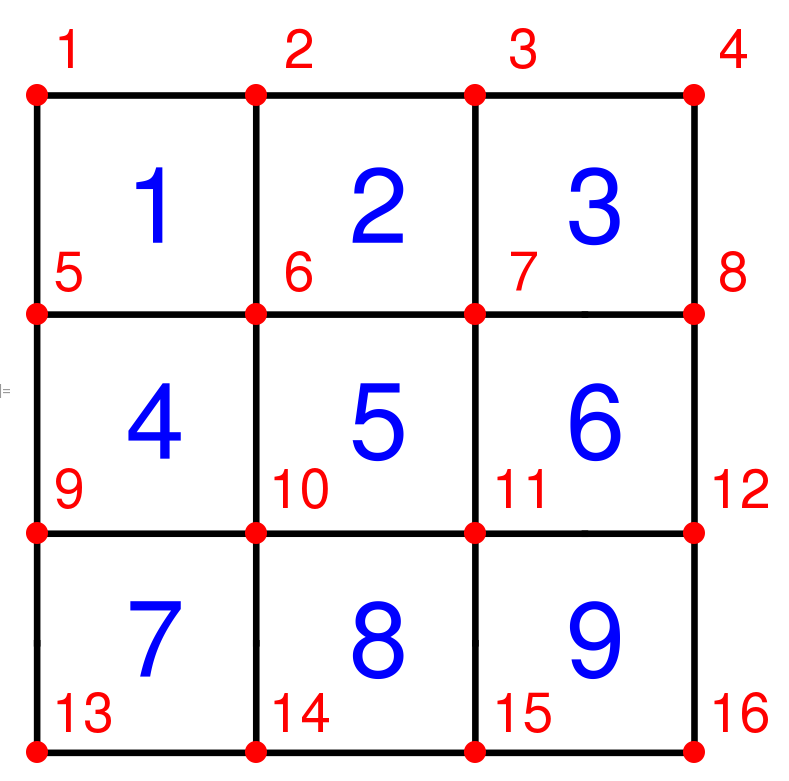
\includegraphics[height=67mm]{Slike/undeformedRegion.png}
        \vspace{6mm}
        \caption{}
    \end{subfigure}
    \begin{subfigure}[b]{0.55\textwidth}
        \centering
        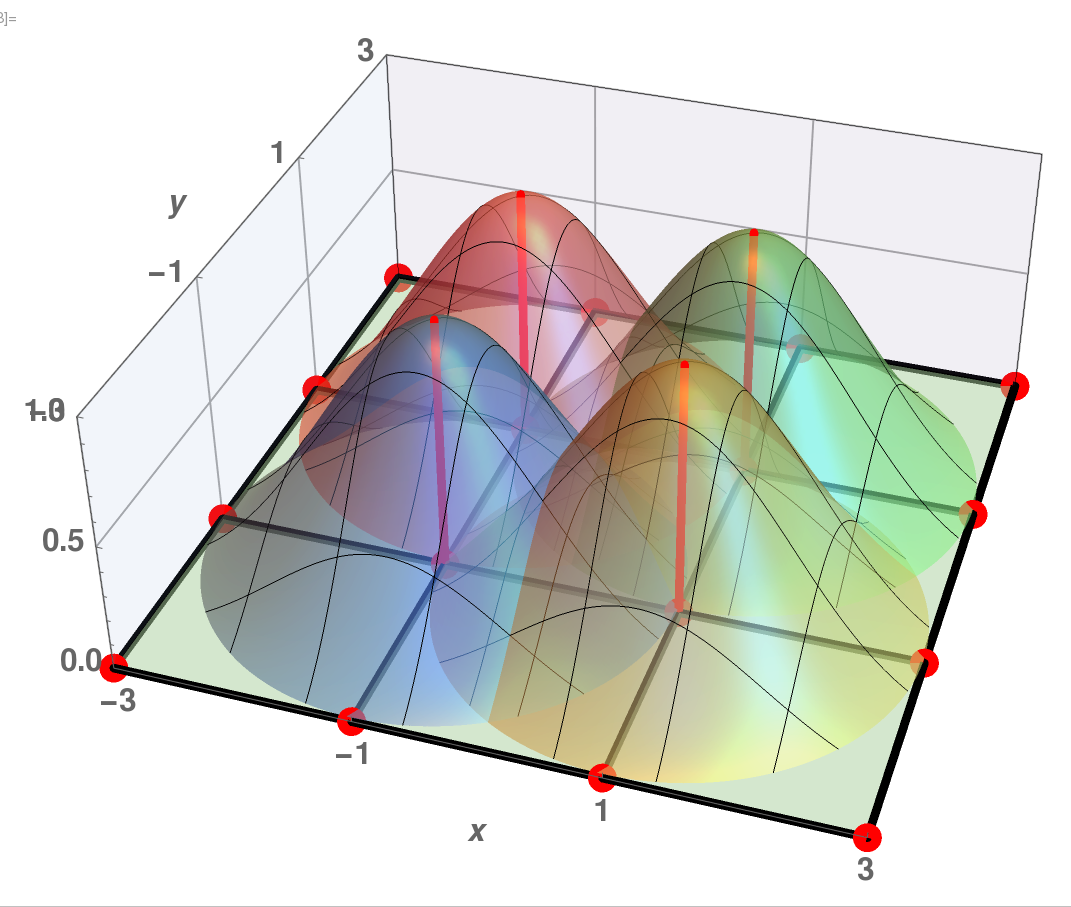
\includegraphics[width=0.94\textwidth]{Slike/undeformedNodeFs.png}
        \caption{}
    \end{subfigure}
    \caption{(a) Pravokotna domena s šestnajstimi vozlišči (rdeče številke) in devetimi elementi (modre številke) ter (b) nad vozlišči napete vozliščne funkcije.}
    \label{fig:regionAndNodeFunctions}
\end{figure}

Vsaka vozliščna funkcija $\Phi_i$ mora pokriti samo elemente, ki se $i$-tega vozlišča dotikajo. S tem dosežemo, da je $v(\bm\chi)$ nad nekim elementom sestavljena le iz funkcij v neposredni bližini tega elementa. Tako je $\mathbf{v}(\bm\chi)$ na sliki \ref{fig:sumAndShapeFunctions}a nad osrednjim elementom popolnoma določena z vrednostmi $v_6, v_7, v_{10}$ in $v_{11}$.

Ozrimo se na variacijsko izjavo \eqref{eq:LsfemVariationalStatement} ter si predstavljajmo funkcije $\mathbsf{A}(\mathbf{x}), \mathbf{u(x)}, \mathbf{v(x)}$ in $\mathbf{f(x)}$ zapisane v smislu razvoja po vozliščnih funkcijah \eqref{eq:nodalSeries}. Zaslutimo, da bomo računali prekrivne integrale vozliščnih funkcij:
\begin{equation}
    \int \mkern-2mu \Phi_i(\mathbf{x}) \mkern4mu \Phi_j(\mathbf{x}) \mkern4mu \ud \Omega \ .
\end{equation}
To je enostavno dokler so vsi elementi iste oblike in velikosti, kot na sliki \ref{fig:regionAndNodeFunctions}. Takrat je dovolj, da izračunamo prekrivne integrale za vozlišča enega elementa. Kaj pa, če želimo uporabljati elemente poljubne oblike? Kako naj čim učinkoviteje, če so elementi poljubne oblike

 Segmente vozliščnih funkcij $\Phi_6, \, \Phi_7, \, \Phi_{10}$ in $\Phi_{11}$, ki se nahajajo neposredno nad elementom 5, proglasimo za \textbf{elementarne funkcije} $\phi_{5 j}(\bm\chi)$ tega elementa (slika \ref{fig:sumAndShapeFunctions}b). Tako lahko funkcijo $\mathbf{v}$ na

\begin{figure}[ht]
    \begin{subfigure}[b]{0.48\textwidth}
        \centering
        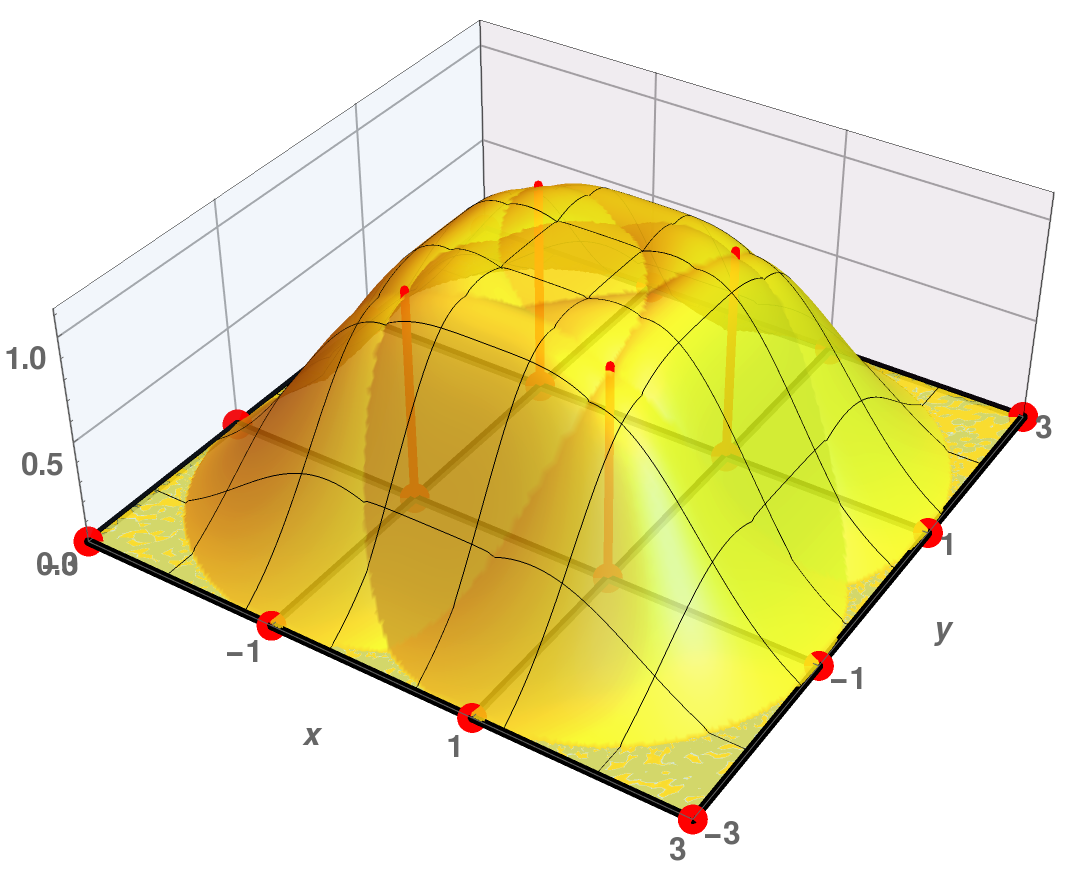
\includegraphics[width=0.94\textwidth]{Slike/sumOfNodeFs.png}
        \vspace{6mm}
        \caption{}
    \end{subfigure}
    \begin{subfigure}[b]{0.48\textwidth}
        \centering
        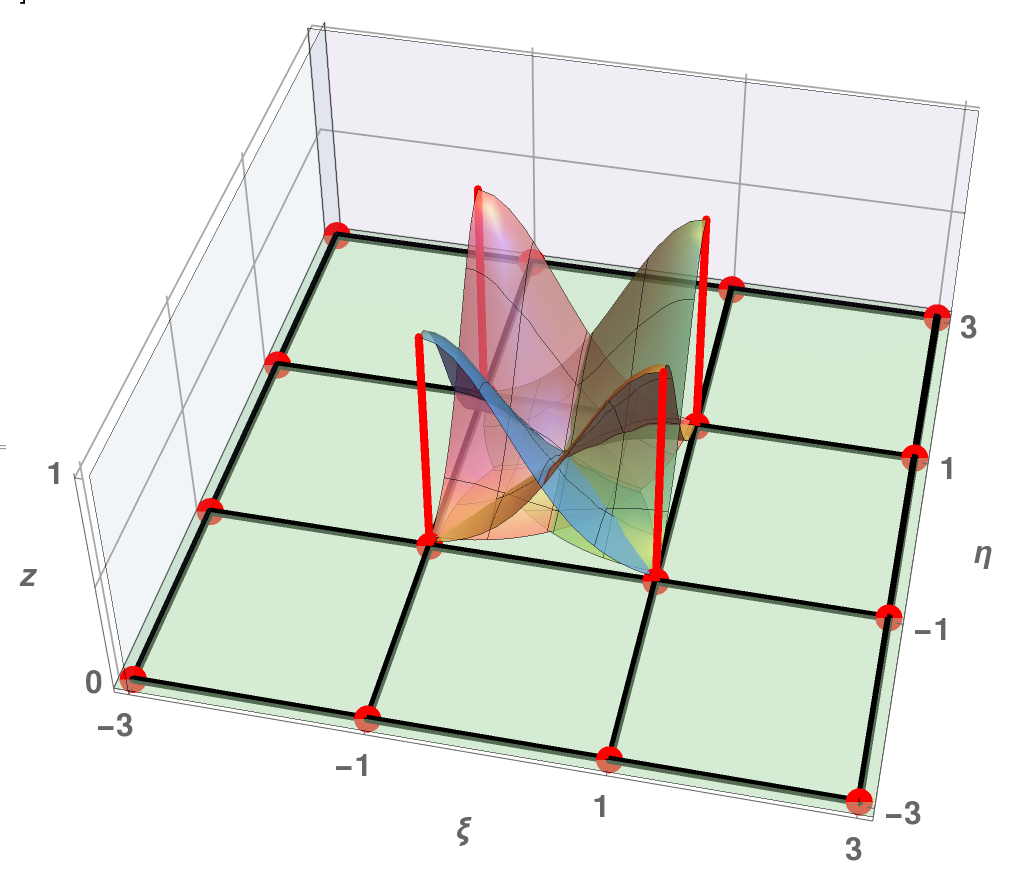
\includegraphics[width=0.94\textwidth]{Slike/undeformedShapeFsFar.png}
        \caption{}
    \end{subfigure}
    \caption{(a) vsota vozliščnih funkcij s slike \ref{fig:regionAndNodeFunctions}b in (b) elementarne funkcije, ki pripadajo elementu 5.}
    \label{fig:sumAndShapeFunctions}
\end{figure}

\begin{figure}[ht]
    \centering
    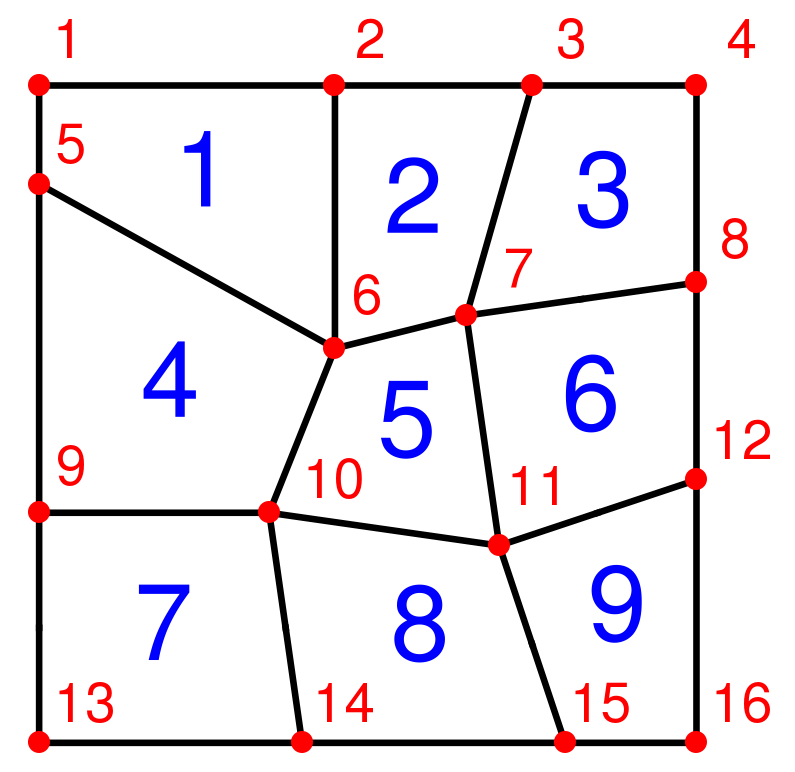
\includegraphics[height=80mm]{Slike/deformedRegion.png}
\end{figure}

\begin{figure}[ht]
    \begin{subfigure}[b]{0.48\textwidth}
        \centering
        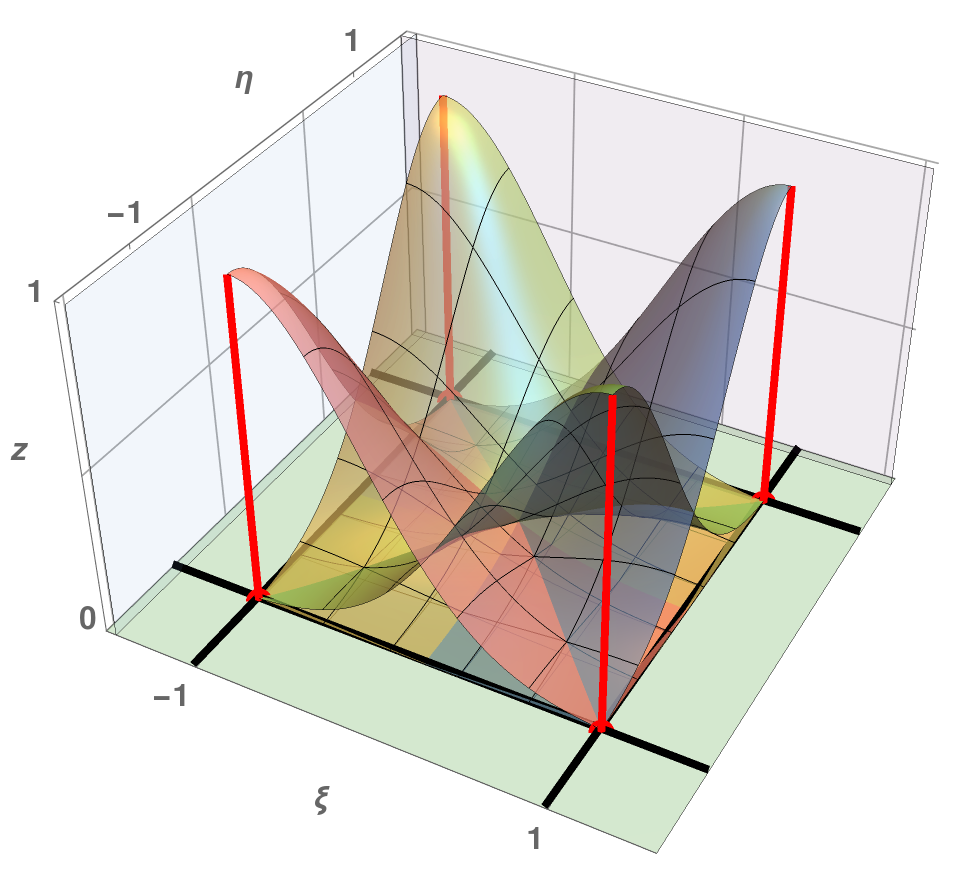
\includegraphics[width=0.94\textwidth]{Slike/undeformedShapeFs.png}
        \vspace{6mm}
        \caption{}
    \end{subfigure}
    \begin{subfigure}[b]{0.48\textwidth}
        \centering
        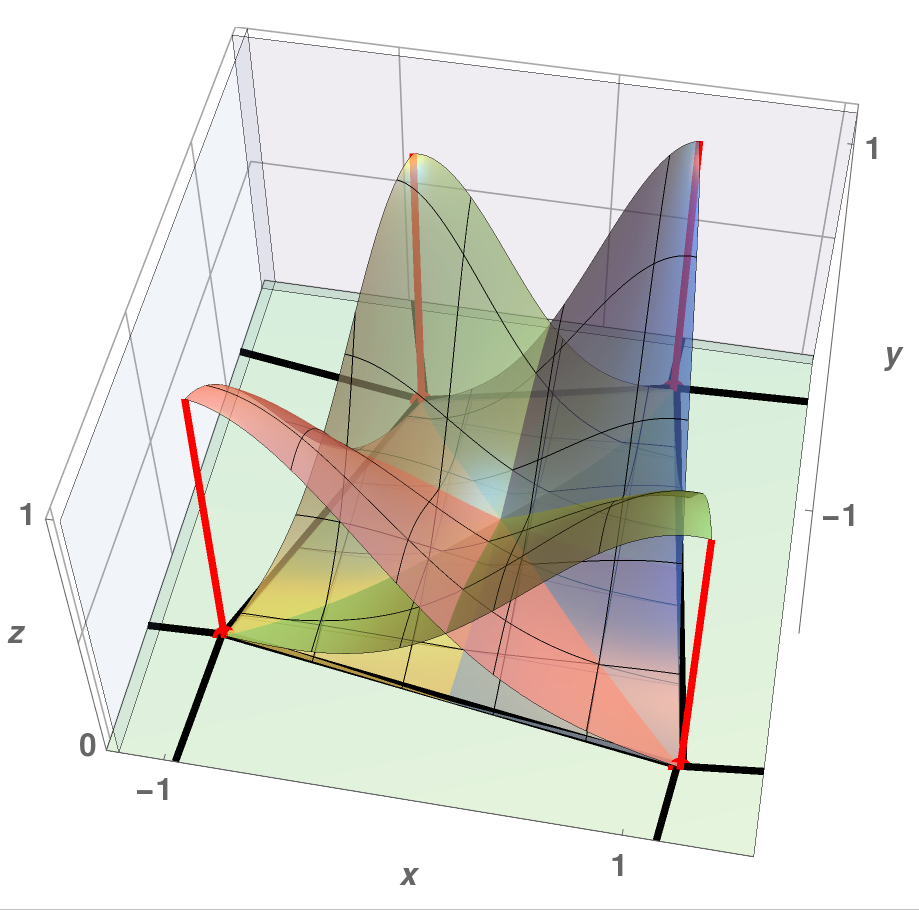
\includegraphics[width=0.94\textwidth]{Slike/deformedShapeFs.png}
        \caption{}
    \end{subfigure}
    \caption{}
    \label{fig:shapeFs}
\end{figure}

še vedno  Z natančno analitično izpeljavo se prebijemo do izjave \eqref{eq:LsfemVariationalStatement}, od tod dalje pa moramo iskanje funkcije $\mathbf{u(x)}$ z neskončno prostostnimi stopnjami poenostaviti v iskanje funkcije s končnim številom prostostnih stopenj $N$. 

Skozi oči \texttt{FI} je $\ket{\Phi_i}$ eden izmed baznih vektorjev v razvoju vektorja $\ket{v}$, $v_i$ pa pripadajoča komponenta.
V jeziku funkcionalne analize (\texttt{FI}) pravimo, da smo omejili funkcijski prostor.

nadaljujemo z diskretizacijo problema, to je, pretvorbo na sistem $N$ algebrajskih enačb. Ta korak je enak pri vseh različicah \texttt{FEM}. Funkcije na domeni $\Omega$ imajo neskončno štveilo prostostnih stopenj. 
\begin{equation}
    u_i(\mathbf{x}) = \sum_{a = 1}^N \Phi^{a0} u^{a0}_i
\end{equation}

Potem omejimo Diskretizacija problema 

Galerkin, Najmanših kvadratov \cite{JiangB-LSFEM}
Basic lemma of variational principles: Temeljni lema variacijskih načel.